\section{Stochastic Differential Equations (SDEs)}

We are trying to solve an equation of the form:
\begin{align}
    dX_t &= b(X_t) \, dt + \sigma(X_t) \, dB_t \\
    X_t &= X_0 + \int_0^t b(X_s) \, ds + \int_0^t \sigma(X_s) \, dB_s
\end{align}

The first integral on the right is a standard Lebesgue/Riemann integral with respect to time, and the second is an Itô integral with respect to Brownian motion.

We are working in a filtered probability space $(\Omega, \mathcal{F}, (\mathcal{F}_t)_{t \ge 0}, P)$, where $B$ is an $(\mathcal{F}_t)$-Brownian Motion. 

There are two main types of solutions we talk about in SDEs:
\begin{itemize}
    \item \textbf{Strong Solution:} The Brownian motion $B$ and the probability space are given in advance, and we need to find $X$ based purely on the information provided by $B$.
    \item \textbf{Weak Solution:} We are only given the functions $b$ and $\sigma$. We are allowed to construct the probability space, the Brownian motion $B$, and the process $X$ all together just to get the statistical distributions to match the equation.
\end{itemize}

In $\R^d$, $X_t$ is a vector, and we have multiple dimensions of noise. We express this using vectors and matrices:
Let $X_t \in \R^d$, the drift vector $b(X_t) \in \R^d$, an $m$-dimensional Brownian motion $B_t \in \R^m$, and the diffusion matrix $\sigma(X_t) \in \R^{d \times m}$. 

In matrix notation, the system looks like this:
\begin{align*}
    \begin{pmatrix}
    dX_t^1 \\ \vdots \\ dX_t^d
    \end{pmatrix}
    =
    \begin{pmatrix}
    b^1(X_t) \\ \vdots \\ b^d(X_t)
    \end{pmatrix} dt
    +
    \begin{pmatrix}
    \sigma_{11}(X_t) & \dots & \sigma_{1m}(X_t) \\
    \vdots & \ddots & \vdots \\
    \sigma_{d1}(X_t) & \dots & \sigma_{dm}(X_t)
    \end{pmatrix}
    \begin{pmatrix}
    dB_t^1 \\ \vdots \\ dB_t^m
    \end{pmatrix}
\end{align*}

Or, written out component-by-component for the $i$-th coordinate:
\begin{align*}
    dX_t^i = b^i(X_t) \, dt + \sum_{j=1}^m \sigma_{ij}(X_t) \, dB_t^j 
\end{align*}

Let's drop back to the deterministic case for a moment. When the noise dimension is $1$ and we completely remove the noise:
\begin{align*}
    \sigma &\equiv 0 \\
    dX_t &= b(X_t) \, dt \\
    X_0 &= x_0 \\
    \frac{d}{dt} X_t &= b(X_t)
\end{align*}
This is just a standard Ordinary Differential Equation (ODE). For ODEs, we mainly care about: does a solution exist, is it unique, and does it survive for all $t > 0$ (global existence) or does it blow up?

\begin{itemize}
    \item \textbf{Picard-Lindelöf Theorem:} If $b$ is globally Lipschitz, a solution exists, is unique, and is defined on the whole real axis $\R$.
    \item \textbf{Peano Theorem:} Only requires $b$ to be continuous. It guarantees a \textit{locally} defined solution exists. However, this solution might not be unique, or it might blow up to infinity in finite time.
\end{itemize}

Here are the classic examples of what goes wrong when $b$ is continuous but not Lipschitz:

\vspace{0.5em}
\noindent\textbf{1. Finite-Time Blowup: $b(x) = x^2$} \\
The solution to $x' = x^2$ with $x(0) = 1$ is $x(t) = \frac{1}{1-t}$. It explodes to infinity as $t \to 1$.

\noindent\textbf{2. Non-Uniqueness: $b(x) = 2\sqrt{|x|}$} \\
The solution to $x' = 2\sqrt{|x|}$ with $x(0) = 0$ can be $x(t) = 0$ forever. But it can also "wake up" at any arbitrary time $c > 0$ and become $x(t) = (t-c)^2$.

\begin{center}
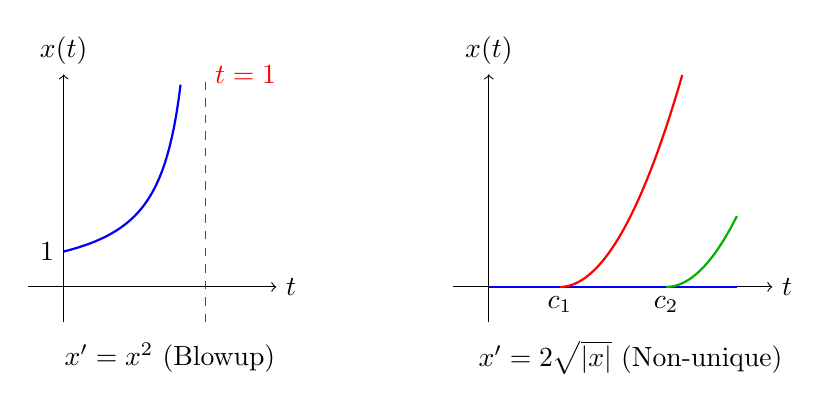
\begin{tikzpicture}[scale=0.9]
    % Graph 1: Blowup
    \draw[->] (-0.5,0) -- (3,0) node[right] {$t$};
    \draw[->] (0,-0.5) -- (0,3) node[above] {$x(t)$};
    \node at (1.5, -1) {$x' = x^2$ (Blowup)};
    \draw[dashed, red] (2,-0.5) -- (2,3) node[right] {$t=1$};
    \draw[thick, blue, domain=0:1.65, samples=100] plot (\x, {1/(2-\x)});
    \node[left] at (0,0.5) {$1$};

    % Graph 2: Non-uniqueness
    \begin{scope}[xshift=6cm]
        \draw[->] (-0.5,0) -- (4,0) node[right] {$t$};
        \draw[->] (0,-0.5) -- (0,3) node[above] {$x(t)$};
        \node at (2, -1) {$x' = 2\sqrt{|x|}$ (Non-unique)};
        
        % Trivial solution
        \draw[thick, blue] (0,0) -- (3.5,0);
        
        % Branching solution 1
        \draw[thick, red, domain=1:2.73, samples=50] plot (\x, {(\x-1)^2});
        \node[below] at (1,0) {$c_1$};
        
        % Branching solution 2
        \draw[thick, green!70!black, domain=2.5:3.5, samples=50] plot (\x, {(\x-2.5)^2});
        \node[below] at (2.5,0) {$c_2$};
    \end{scope}
\end{tikzpicture}
\end{center}

Now, back to stochastics:

\begin{definicija}
    We say that the functions $b$ and $\sigma$ are \textit{K-Lipschitz} (globally) if there exists a constant $K$ such that for all $x, y$:
    \begin{align*}
        \| b(x) - b(y) \| + \| \sigma(x) - \sigma(y) \| \leq K \| x-y \|
    \end{align*}
\end{definicija}

\begin{izrek}[Existence and Uniqueness of SDEs]
    Given a filtered probability space and $B$ an $(\mathcal{F}_t)$-Brownian Motion, assume $b$ and $\sigma$ are globally Lipschitz. 
    
    Then for every initial value $x_0 \in \R^d$, there exists a continuous semimartingale $X$ such that:
    \begin{align}
        \forall t \geq 0, \quad X_t = x_0 + \int_0^t b(X_s) \, ds + \int_0^t \sigma(X_s) \, dB_s
        \label{eq:sde1}
    \end{align}
    This means a \textbf{global solution exists}.

    If $Y$ is another continuous semimartingale solving this same equation, then $P(X_t = Y_t \text{ for all } t) = 1$. This means the solution is \textbf{unique}.

    Finally, the solution $X$ is adapted to the filtration generated by $B$. \\
    \textit{(What this means: This is exactly what makes it a "strong solution". It implies that if you know the exact path the noise $B$ took up to time $t$, you have all the information you need to completely determine the exact path of $X$ up to time $t$. The noise purely dictates the outcome.)}
\end{izrek}

\textbf{Markov Property:} For $x \in \R^d$, let $\mathcal{L}_x$ be the probability law of the unique solution to \eqref{eq:sde1} starting at $X_0 = x$. Then for any $t_0 \geq 0$ and $t \ge 0$, the conditional law of $X_{t_0+t}$ given the history $\mathcal{F}_{t_0}$ is simply $\mathcal{L}_{X_{t_0}}$. 
In short: the future only depends on the present state $X_{t_0}$, not on how it got there.

\obvs
(At least it's obvious to me. Maybe the rigorous proof is highly technical, but the intuition is clear!)

Just like with ODEs, the proof of the existence theorem relies on \textbf{Picard Iterations}. We define a sequence of processes $(X^n)_{n \geq 0}$:
\begin{align*}
    X_t^0 &= x_0 \\
    X_t^1 &= x_0 + \int_0^t b(X_s^0) \, ds + \int_0^t \sigma(X_s^0) \, dB_s \\
    X_t^2 &= x_0 + \int_0^t b(X_s^1) \, ds + \int_0^t \sigma(X_s^1) \, dB_s \\
    &\vdots \\
    X_t^n &= x_0 + \int_0^t b(X_s^{n-1}) \, ds + \int_0^t \sigma(X_s^{n-1}) \, dB_s
\end{align*}

We want to show that this sequence forms a contraction in a suitable space of functions, which will mean that there is a unique fixed point $X^\infty_t$ that is well-defined and perfectly satisfies the SDE. 

To prove this contraction works, we need two main tools:

\begin{lema}[Grönwall's Inequality]
    Let $f: [0, T] \to [0, \infty)$ be a bounded, measurable, non-negative function. If there exists a constant $c > 0$ such that for all $t \in [0, T]$:
    \begin{align*}
        f(t) \leq c \int_0^t f(s) \, ds
    \end{align*}
    Then $f(t) = 0$ for all $t$.
\end{lema}

\begin{proof}
    Consider the function $v(t) = \exp(-ct) \int_0^t f(s) \, ds$. If we take the derivative of $v$:
    \begin{align*}
        v'(t) &= -c \exp(-ct) \int_0^t f(s) \, ds + \exp(-ct) f(t) \\
              &= \exp(-ct) \left( f(t) - c \int_0^t f(s) \, ds \right)
    \end{align*}
    Because of our assumption, the term in the parentheses is $\leq 0$. Therefore, $v'(t) \leq 0$, meaning $v$ is decreasing. We know $v(0) = 0$, so $v(t) \leq 0$ for all $t \geq 0$. But since $f$ is non-negative, $v(t)$ must also be non-negative. The only way it can be both $\leq 0$ and $\geq 0$ is if $v(t) = 0$. This forces $f(t) = 0$ everywhere.
\end{proof}

\begin{lema}[Banach Fixed-Point Theorem]
    Let $(E, d)$ be a complete metric space and $F: E \to E$ be a mapping. If there exists an integer $n > 0$ and a constant $\lambda \in (0, 1)$ such that for all $x, y \in E$:
    \begin{align*}
        d(F^n(x), F^n(y)) \leq \lambda \, d(x,y)
    \end{align*}
    (Often we just need $n=1$ and $\lambda = \frac{1}{2}$). 
    Then $F$ has a unique fixed point in $E$, meaning there is exactly one $x^*$ such that $F(x^*) = x^*$.
\end{lema}

\obvs

\begin{proof}[Proof: Uniqueness and Existence via Picard Iterations]
    Let's assume $d=1$. Since $\sigma$ and $b$ are globally $K$-Lipschitz, they also satisfy a linear growth bound. We can see this by adding and subtracting $0$:
    \begin{align*}
        |\sigma(x)| &= |\sigma(x) - \sigma(0) + \sigma(0)| \leq |\sigma(0)| + K|x| \\
        |b(x)| &= |b(x) - b(0) + b(0)| \leq |b(0)| + K|x|
    \end{align*}

    \textbf{Step 1: Uniqueness} \\
    Assume $X$ and $Y$ are both solutions to the SDE with the same initial value $X_0 = Y_0 = x_0$. We define a stopping time $F_n = \inf\{t \geq 0 : |X_t| \geq n \text{ or } |Y_t| \geq n\}$ to keep our processes bounded, and look at a fixed time horizon $T$. 
    
    We want to show that the expected squared difference is zero:
    \begin{align*}
        E\left[(X_{t \wedge F_n} - Y_{t \wedge F_n})^2\right] = E \left[ \left( \int_0^{t \wedge F_n} \big(b(X_s) - b(Y_s)\big) ds + \int_0^{t \wedge F_n} \big(\sigma(X_s) - \sigma(Y_s)\big) dB_s \right)^2 \right]
    \end{align*}
    
    Using the inequality $(A+B)^2 \leq 2A^2 + 2B^2$, we can split the drift and diffusion parts:
    \begin{align*}
        E\left[(X_{t \wedge F_n} - Y_{t \wedge F_n})^2\right] \leq 2 E \left[ \left( \int_0^{t \wedge F_n} \big(b(X_s) - b(Y_s)\big) ds \right)^2 \right] + 2 E \left[ \left( \int_0^{t \wedge F_n} \big(\sigma(X_s) - \sigma(Y_s)\big) dB_s \right)^2 \right]
    \end{align*}

    For the first part (the drift), we use the Cauchy-Schwarz inequality for integrals: $\left(\int_0^t f(s) ds\right)^2 \leq t \int_0^t f(s)^2 ds$. Together with the Lipschitz property of $b$, we get:
    \begin{align*}
        2 E \left[ \left( \int_0^{t \wedge F_n} \big(b(X_s) - b(Y_s)\big) ds \right)^2 \right] 
        &\leq 2t E \left[ \int_0^{t \wedge F_n} \big(b(X_s) - b(Y_s)\big)^2 ds \right] \\
        &\leq 2T K^2 \int_0^t E \left[ (X_{s \wedge F_n} - Y_{s \wedge F_n})^2 \right] ds
    \end{align*}

    For the second part (the diffusion), we use the magical \textbf{Itô Isometry}, which turns the expected square of an Itô integral into a standard Riemann integral: $E[(\int f dB_s)^2] = E[\int f^2 ds]$. Using the Lipschitz property of $\sigma$:
    \begin{align*}
        2 E \left[ \left( \int_0^{t \wedge F_n} \big(\sigma(X_s) - \sigma(Y_s)\big) dB_s \right)^2 \right] 
        &= 2 E \left[ \int_0^{t \wedge F_n} \big(\sigma(X_s) - \sigma(Y_s)\big)^2 ds \right] \\
        &\leq 2 K^2 \int_0^t E \left[ (X_{s \wedge F_n} - Y_{s \wedge F_n})^2 \right] ds
    \end{align*}

    Putting both bounds together and factoring out the integral gives:
    \begin{align*}
        E\left[(X_{t \wedge F_n} - Y_{t \wedge F_n})^2\right] \leq 2 K^2 (T + 1) \int_0^t E \left[ (X_{s \wedge F_n} - Y_{s \wedge F_n})^2 \right] ds
    \end{align*}

    This is exactly the setup for Grönwall's Lemma! Let $f(t) = E[(X_{t \wedge F_n} - Y_{t \wedge F_n})^2]$ and $C = 2 K^2 (T + 1)$. We have $f(t) \leq C \int_0^t f(s) ds$, which forces $f(t) = 0$ for all $t$. Taking the limit as $n \to \infty$, we conclude $X_t = Y_t$ almost surely.

    \vspace{1em}
    \textbf{Step 2: Existence} \\
    To prove existence, we need to show that our Picard iteration is a contraction. Define the mapping $\Phi$ taking a process $Y$ to a new process:
    \begin{align*}
        \Phi(Y)_t = x_0 + \int_0^t b(Y_s) ds + \int_0^t \sigma(Y_s) d B_s
    \end{align*}

    We calculate the expected squared distance between $\Phi(X)$ and $\Phi(Y)$ at time $t$. Using the exact same $(A+B)^2$ trick, Cauchy-Schwarz, Itô Isometry, and Lipschitz bounds as we did for uniqueness, we get the exact same bound:
    \begin{align*}
        E\left[|\Phi(X)_t - \Phi(Y)_t|^2\right] \leq 2 K^2 (T + 1) \int_0^t E\left[|X_s - Y_s|^2\right] ds
    \end{align*}

    Let $C = 2 K^2 (T + 1)$ and define the maximum expected distance over the interval $[0, T]$ as our metric $d(X,Y)^2$. If we plug the bound back into itself (iterating the map), we start picking up factorials from the time integral:
    \begin{align*}
        E\left[|\Phi^2(X)_t - \Phi^2(Y)_t|^2\right] &\leq C \int_0^t C \int_0^s E\left[|X_u - Y_u|^2\right] du \, ds \leq \frac{C^2 t^2}{2} d(X, Y)^2 \\
        &\vdots \\
        E\left[|\Phi^n(X)_t - \Phi^n(Y)_t|^2\right] &\leq \frac{(C t)^n}{n!} d(X, Y)^2
    \end{align*}
    
    Since factorials grow much faster than exponential powers, $\frac{(CT)^n}{n!} \to 0$ as $n \to \infty$. So, for a large enough $n$, this fraction is strictly less than $\frac{1}{2}$. 
    
    This means $\Phi^n$ is a strict contraction! By the Banach Fixed Point Theorem, there exists a unique fixed point $X$ such that $\Phi(X) = X$, which is exactly our guaranteed strong solution.
\end{proof}